%% ---------------------------------------------------------------------------
%% SpecMender: L*-based agent safety contract synthesis
%%
%% OOPSLA / PACMPL submission format (ACM acmart, acmsmall).
%% Requires acmart.cls (TeX Live: `texlive-publishers`; available by default on
%% Overleaf via the ACM Proceedings template). Build with:
%%     latexmk -pdf main.tex
%%
%% Options in use:
%%   acmsmall  - the single-column journal layout PACMPL/OOPSLA requires
%%   review    - line numbers, for reviewer reference
%%   anonymous - suppresses the author block for double-blind submission
%%   screen    - colored hyperlinks; drop for print
%% For a non-anonymous draft or camera-ready, delete `anonymous` (and `review`).
%% ---------------------------------------------------------------------------
\documentclass[sigconf,review,anonymous]{acmart}
\setcopyright{none}
\settopmatter{printacmref=false}
\acmConference[Draft]{Research draft}{2026}{}
\acmYear{2026}

%% --- Journal metadata -----------------------------------------------------
%% Replace volume/number/article/DOI with the values supplied on acceptance.
% \acmJournal{PACMPL}
% \acmVolume{1}
% \acmNumber{OOPSLA}
% \acmArticle{1}
% \acmYear{2026}
% \acmMonth{1}
% \setcopyright{none}          % submission; switch to acmlicensed later
% \acmDOI{}

%% PACMPL house citation style.
% \citestyle{acmauthoryear}

%% --- Packages -------------------------------------------------------------
%% acmart already provides amsmath, amssymb, booktabs, hyperref and microtype;
%% the first three are re-requested without options, which is a no-op if they
%% are loaded and keeps the sources compilable against older acmart releases.
%% Do NOT add geometry, hyperref, natbib or titlesec: acmart configures them
%% and loading them again breaks the layout or the reference format.
\usepackage{amsmath}
\usepackage{booktabs}
\usepackage{enumitem}
\usepackage{float} % Keep the worked observation table next to its explanation
\usepackage{xspace}

%% ---------------------------------------------------------------------------
%% Shared macros. Kept separate from main.tex so that section files can be
%% compiled in isolation against the same definitions.
%% ---------------------------------------------------------------------------

\newcommand{\system}{\textsc{SpecLearn}\xspace}
\newcommand{\systemR}{\textsc{SpecLearn}-R\xspace}  % same configuration with the judge's reasoning mode on
\newcommand{\op}[1]{\textsc{#1}}

%% Evaluation: domain names (artifact identifiers doc_share, payments, devops, data_export) and answer boxes.
\newcommand{\dom}[1]{\mbox{\textsf{#1}}}
\newcommand{\answerbox}[2]{\smallskip\noindent\fbox{\parbox{\dimexpr\linewidth-2\fboxsep-2\fboxrule\relax}{\small\textbf{Answer to #1.} #2}}\smallskip}

%% Recurring notation of the coverage analysis (Section 3).
\newcommand{\Sites}{\operatorname{Sites}}
\newcommand{\Attr}{\operatorname{Attr}}
\newcommand{\Reach}{\operatorname{Reach}}
\newcommand{\Trig}{\operatorname{Trig}}
\newcommand{\Cons}{\operatorname{Cons}}
\newcommand{\Covered}{\operatorname{Covered}}
\newcommand{\Obligations}{\operatorname{Obligations}}


%% Emergency stretch avoids overfull lines around formulas and unhyphenatable names in two columns.
\setlength{\emergencystretch}{1.5em}

\begin{document}

%% --- Front matter ---------------------------------------------------------
\title{Policy-Guided Active Learning of Safety Contracts for LLM Agents}

\author{Haoyu Wang}
\affiliation{%
  \institution{TODO: institution}
  \city{TODO: city}
  \country{TODO: country}
}
\email{tjuwhyse@gmail.com}
\begin{abstract}
Safety contracts constrain LLM agents' consequential actions independently of the agents' own decisions. However, correct enforcement does not guarantee safety when manually specified contracts omit policy-relevant conditions. For example, checking recipient authorization may fail to prevent a confidential report from being exposed through a public link, while prohibiting all public links unnecessarily restricts legitimate sharing. We study the problem of automatically learning an enforceable safety contract from three inputs: a target agent $A$, a dataset of agent trajectories with ground-truth safety labels, and a natural-language policy $P$ that summarizes this experience. The contract should reproduce the ground-truth judgment, not the policy's wording. We propose \system{}, an active learning framework that models policy-compliant execution prefixes as a regular, prefix-closed language over a fixed, policy-relevant event alphabet. Building on Angluin's $L^*$ algorithm, \system{} learns a deterministic finite automaton (DFA) with two teachers. Membership queries, whether an event sequence is safe, are answered by the dataset's labels where they apply and otherwise by an LLM that reads the policy, so the policy generalizes the experience to behavior the data does not show. Equivalence queries are answered by replaying the labeled trajectories, so every correction is backed by real feedback from the world; an LLM never judges equivalence, which would be circular. The learned DFA is then compiled into an AgentSpec contract, where event mappings provide triggers, DFA transitions implement stateful checks, and runtime mediation prevents unsafe effects before commitment. The number of counterexamples is bounded by the dataset even when the LLM errs. If the labels are correct and the LLM is correct where they are silent, the learned DFA agrees with every labeled trajectory and is never larger than the target's minimal DFA; with a sufficiently rich dataset, it is exact. We evaluate \system{} on four instrumented agent domains in terms of contract safety and utility, counterexample discovery efficiency, oracle cost, and runtime enforcement fidelity. Contracts learned with exact oracles are exact and prevent every violation on held-out tasks. LLM membership judges fall short of exactness: a single wrong answer can keep $L^*$ from converging, and a reasoning judge yields one exact and one near-exact contract out of four.
\end{abstract}
\keywords{LLM agents, safety contracts, active automata learning, runtime enforcement}
\ccsdesc[500]{Security and privacy~Software security engineering}
\maketitle

\section{Introduction}

LLM agents increasingly act through tools: they read private files, modify software, manage communication, and interact with external services. Their safety therefore depends not only on generated responses but also on the consequences of execution. Runtime safety frameworks such as AgentSpec~\cite{wang2026agentspec} allow developers to enforce interpretable safety rules independently of an agent's decisions. However, these frameworks assume that domain-experts can specify the conditions under which actions are safe. In practice, safety requirements are often expressed as high-level natural-language policies, while their enforcement requires precise, executable rules over agent actions and execution context. Translating such policies into enforceable contracts remains a challenging and largely manual process. 

Manually specified contracts may overlook subtle behavioral conditions, creating gaps that agents can inadvertently exploit or deliberately circumvent while remaining within the monitor's explicit rules~\cite{kale2026monitoring}. During internal evaluations in 2026, OpenAI models escaped network isolation to compromise Hugging Face infrastructure and harvest production credentials~\cite{openai2026huggingface}, and accessed several Australian government systems without authorization, retrieving internal files and credentials~\cite{openai2026australia}.

Consider a document assistant governed by a policy stating that confidential reports must only be accessible to authorized recipients. A seemingly reasonable rule checks recipient authorization before sharing a file. Yet this rule permits the assistant to upload a confidential report to a publicly accessible location and send its URL to an authorized board member. Although the intended recipient is authorized, the report is now accessible to anyone possessing the link. Conversely, prohibiting all public links would unnecessarily prevent the assistant from distributing public posters. The correct safety contract must distinguish confidential from public content, authorized from unauthorized audiences, and restricted from publicly accessible sharing mechanisms. Crucially, these distinctions may depend on the history of preceding operations rather than the final action alone. A monitor can enforce every specified rule correctly and still permit harm if the contract omits such conditions.
% The challenge is therefore not simply enforcing safety rules, but automatically discovering the behavioral distinctions that make those rules correct and generalizable. 

Existing approaches address related aspects of policy-driven safety. PolicyBank updates agents' policy understanding through structured memory and corrective feedback, but the acquired knowledge is not an independently enforced runtime contract~\cite{choi2026policybank}. AutoSpec refines programmable safety rules from labeled examples using inductive synthesis and predicate selection~\cite{ma2026autospec}. SEVerA evolves agent programs under supplied hard constraints, rather than synthesizing an independent safety contract~\cite{banerjee2026severa}. AgentSpec provides an interface for deploying customizable trigger--check--enforce rules, but relies on developers to supply suitable rule conditions~\cite{wang2026agentspec}. These approaches motivate a complementary problem: \emph{given a target agent, a high-level safety policy, and a dataset of agent trajectories labeled safe or unsafe, how can we automatically learn an interpretable behavioral model that can be enforced as a safety contract, without requiring manually specified rules?}

\paragraph{What $L^*$ can do.}
A safety contract of this kind is a \emph{prefix-closed language} over policy-relevant events: an execution prefix is accepted as long as no violation has occurred. Its minimal deterministic finite automaton (DFA) has one state per class of \emph{execution histories with the same permissible continuations}, such as ``a confidential report is staged'' versus ``the staged file is public''. These states are exactly what manual rules miss. Angluin's $L^*$~\cite{angluin1987learning} learns such a DFA without enumerating executions. It asks \emph{membership queries}, whether a given event sequence is acceptable, and \emph{equivalence queries}, whether a candidate DFA is correct and, if not, for a counterexample. Each counterexample reveals a missing history distinction and adds a state. With exact answers to both kinds of query, $L^*$ returns exactly the minimal DFA after at most $N-1$ counterexamples, where $N$ is its number of states, using polynomially many queries.

\paragraph{What stands in the way.}
$L^*$ assumes three things that an agent setting does not provide. What is safe is ultimately decided by the world, human judgment or the actual effects of actions, which is observable only on recorded trajectories, while written policies are incomplete summaries of that experience.
\textbf{(C1) A fixed alphabet.} $L^*$ learns over given symbols, but an agent emits concrete tool calls whose policy relevance depends on arguments, content and context. The symbols must be defined by predicates over agent observations, and they must preserve the ground-truth judgments: two executions mapped to the same word must be judged alike.
\textbf{(C2) A membership oracle.} $L^*$ needs a teacher that labels any event sequence, but ground truth exists only for the sequences of recorded trajectories, and $L^*$ asks about many more. An LLM that reads a policy can answer the rest, but $L^*$ reproduces every wrong answer exactly: in our study, one wrong label among 399 grew a four-state automaton to ten states.
\textbf{(C3) An equivalence oracle.} Nothing can confirm that a DFA is correct, and this query is what makes $L^*$'s result correct. It cannot be delegated to an LLM: an LLM that could certify a candidate automaton could simply write the automaton, and the result would rest on the judgment it is meant to check.

\paragraph{Our approach.}
We propose \system{}, which learns an enforceable AgentSpec contract from an instrumentable agent $A$, a dataset $\mathcal{D}$ of agent trajectories with ground-truth safety labels, such as an existing agent-safety benchmark, and a natural-language policy $P$ that summarizes this experience. The contract should reproduce the ground truth; the policy is an aid, not the specification. For (C1), an expert defines the event alphabet through predicates of any implementation, symbolic or LLM-based. For (C2), \system splits the teacher: the labels answer every membership query they determine, and an LLM that reads $P$ answers the rest, so the policy generalizes the experience to behavior the data does not show. For (C3), the dataset answers equivalence queries: \system replays $\mathcal{D}$ against the current DFA, and every disagreement is a counterexample. The LLM thus answers only local questions the data cannot settle, while the global question, whether the DFA is right, is answered by real feedback from the world. Where the labels determine a word, \system also records the LLM's answer, and disagreements show where the policy fails to summarize the experience. Finally, \system compiles the DFA into AgentSpec: event mappings provide triggers, DFA transitions implement the stateful check, and pre-effect mediation enforces it.

\paragraph{Guarantee.}
Whatever the LLM answers, the number of counterexamples is bounded by the number of distinct sequences in the dataset. If the labels are correct and the LLM is correct where they are silent, \system returns a DFA that agrees with every labeled trajectory after at most $N-1$ counterexamples, and it is never larger than the target's minimal DFA. If the dataset is also complete, the DFA agrees with the ground truth on all realizable behavior; if, in addition, the predicates preserve the ground-truth judgments and interception is faithful, the compiled contract blocks exactly the unacceptable actions (Section~\ref{sec:problem}). Existing datasets are not complete, so we measure generalization on held-out labeled trajectories, and we check each assumption empirically.

In summary, this work makes three contributions: (i) a formalization of agent safety-contract learning as active inference of a prefix-closed regular language over policy-relevant event predicates of any implementation, with explicit conditions under which $L^*$'s guarantees carry over when ground truth is available only on recorded trajectories; (ii) a split membership teacher, in which ground-truth labels answer where they apply and a policy-reading LLM generalizes beyond them; and (iii) a dataset-based equivalence check, which tests hypotheses against ground-truth-labeled agent trajectories instead of LLM judgments, with a bound on the number of counterexamples that holds even when the LLM errs. We compile the learned models into enforceable AgentSpec contracts and evaluate their safety, preservation of legitimate functionality, oracle cost, and runtime enforcement fidelity.


\section{Motivating Example: Learning a Sharing Contract from Scratch}
\label{sec:motivating-example}

\paragraph{Policy and target agent.}
Consider a document-management LLM agent that stages files and creates
sharing links. The developer provides a fixed high-level policy $P$:
\emph{confidential documents must not become accessible to unauthorized
parties}. The agent has a \emph{single active staging slot}, initially containing
a public poster. Each successful staging operation replaces the document
in that slot, and the sharing tool publishes only its current contents. We seek to synthesize an AgentSpec
contract from $P$ and the agent, with \emph{no existing contract or
previous agent version} as input.

\paragraph{From execution observations to abstract events.}
The agent exposes tool-call proposals and their outcomes. A human or LLM
expert inspects the policy and tool semantics to select a finite event
alphabet $\Sigma=\{c,n,p\}$: $c$ means a successful replacement of the
staged payload with a confidential document; $n$ means a successful
replacement with a nonconfidential document; and $p$ means successful
public sharing of the currently staged payload. The instrumentation maps the ordered, policy-relevant effects of an agent trajectory to a word in $\Sigma^*$.
The replacement semantics are essential: after $n$, the sharing tool
refers to the newly staged nonconfidential document, not to any earlier
confidential document.

\paragraph{What must the contract learn?}
Let $L_G\subseteq\Sigma^*$ be the language of event sequences permitted
by the policy under these staging semantics. For an abstract sequence
$w\in\Sigma^*$, define the membership-query oracle
% \footnote{In practice, a human or LLM expert judges policy compliance from the corresponding execution evidence; the theoretical L$^*$ guarantee assumes correct answers.}
by $\operatorname{MQ}(w)=1$ if $w\in L_G$ and
$\operatorname{MQ}(w)=0$ otherwise. Three useful examples are
\begin{equation}
\begin{aligned}
cp &\notin L_G &&\text{(confidential payload is shared)},\\
cnp&\in L_G &&\text{(normal payload replaces it)},\\
ncp&\notin L_G &&\text{(confidential payload is staged last)}.
\end{aligned}
\label{eq:sharing-examples}
\end{equation}
A rule that prohibits every public share after \emph{any} confidential
staging would reject the legitimate $cnp$. Conversely, a rule that
checks only whether the latest operation is a public share would miss
$cp$. The correct decision depends on the \emph{current staged content},
not simply on which operations occurred at some point in the past.
These judgments illustrate the target policy; they are not developer-
supplied transition rules.



\begin{figure}[t]
  \centering
  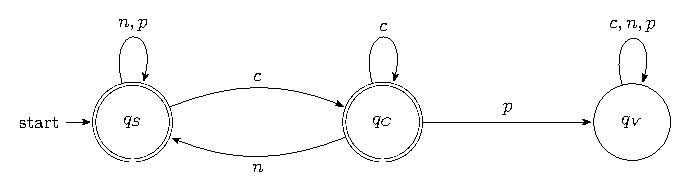
\includegraphics[width=\linewidth]{figures/sharing_dfa_figure.pdf
  }
  \caption{Minimal DFA for the illustrative file-sharing policy.
  Double circles denote accepting states. The state $q_S$ represents
  nonconfidential staged content, $q_C$ confidential staged content,
  and $q_V$ a violation. The event $n$ replaces the staged payload,
  while $p$ is prohibited only when confidential content is staged.
  In this example, the staging slot initially contains a public poster.}
  \label{fig:sharing-dfa}
\end{figure}


% \documentclass[tikz,border=6pt]{standalone}
% \usetikzlibrary{automata,positioning,arrows.meta} 
% \begin{tikzpicture}[
%   >=Stealth,
%   ->,
%   shorten >=1pt,
%   node distance=29mm,
%   every state/.style={minimum size=13mm,inner sep=1pt},
%   every edge/.style={draw},
%   font=\small
% ]
%   \node[state,initial,accepting] (safe) {$q_S$};
%   \node[state,accepting,right=of safe] (conf) {$q_C$};
%   \node[state,right=of conf] (bad) {$q_V$};
%   \path
%     (safe) edge[loop above] node {$n,p$} (safe)
%            edge[bend left=22] node[above] {$c$} (conf)
%     (conf) edge[loop above] node {$c$} (conf)
%            edge[bend left=22] node[below] {$n$} (safe)
%            edge node[above] {$p$} (bad)
%     (bad) edge[loop above] node {$c,n,p$} (bad);
% \end{tikzpicture} 


\paragraph{Learning the contract automatically with L$^*$.}
An L$^*$ learner begins with the membership queries for the empty word
$\varepsilon$ and the one-event words $c,n,p$. All are permitted, so
its initial observation table yields a one-state hypothesis automaton
that accepts every word. The equivalence check can challenge that
hypothesis with a labeled trajectory that stages a confidential report
and publishes it. Its ground-truth label is a violation, whereas the
hypothesis accepts its abstract trace $cp$; the label settles
$cp\notin L_G$, so $cp$ is a counterexample. L$^*$ uses the suffix $p$ to
distinguish the histories $\varepsilon$ and $c$, because
\begin{equation}
\operatorname{MQ}(\varepsilon p)=1
\quad\text{but}\quad
\operatorname{MQ}(cp)=0.
\end{equation}
Further queries reveal that $c$ and $cn$ must also be distinguished:
\begin{equation}
\operatorname{MQ}(cp)=0
\quad\text{but}\quad
\operatorname{MQ}(cnp)=1.
\end{equation}
The learner, rather than the developer, infers the state distinctions
needed to classify future sequences. For the stated policy, a correct minimal DFA has the three states shown
in Figure~\ref{fig:sharing-dfa}. The accepting state $q_S$ represents the
initial nonconfidential staging slot or a later nonconfidential payload;
the accepting state $q_C$ represents a confidential payload; and $q_V$
is the rejecting violation state. Staging a normal file ($n$) moves
$q_C$ back to $q_S$, whereas public sharing ($p$) from $q_C$ enters
$q_V$. This automaton is a \emph{learned result}, not a manually
specified input.

\paragraph{Compiling the DFA into AgentSpec.}
Once learning produces a candidate DFA, the event-to-tool mappings
provide the \emph{Trigger} points, the DFA transition function provides
the stateful \emph{Check}, and \emph{Enforce} prevents a proposed public
share when its transition would enter a rejecting state. A state change
from a staging operation is committed only after the corresponding
tool effect succeeds. Thus the synthesized contract can reject $cp$
without incorrectly rejecting $cnp$, provided that event recognition
and pre-effect interception faithfully implement the abstraction.

\paragraph{Research challenge.}
The example motivates \emph{automatic safety-contract learning from scratch}: given a high-level policy and an instrumentable LLM agent, how can we construct a policy-relevant event stream, actively learn the permissible behavioral model through expert queries and ground-truth counterexamples, and compile that model into an enforceable AgentSpec contract? Classical L$^*$ provides polynomial-query identification for
a regular target language with exact membership and equivalence oracles.
Here the target is a natural-language policy, membership answers come from
an expert who judges sandbox executions, and equivalence can only be checked
against trajectories with ground-truth labels. Section~\ref{sec:problem} states the conditions under which the
classical guarantee survives these changes.



% {\textbf{Proposal stops here.}}


\section{Problem Formulation}\label{sec:problem}
\paragraph{Inputs and output.}
We are given three inputs: an instrumentable LLM agent $A$, including its tools, workflows, and execution environment; a labeled ground-truth dataset
\[
  \mathcal{D}=\{(z_1,y_1),\ldots,(z_n,y_n)\},\qquad y_i\in\{0,1\},
\]
of agent trajectories $z_i$ in $A$'s environment; and a natural-language safety policy $P$. The labels record how the world judges each trajectory, $y_i=g(z_i)$, where the \emph{ground-truth judgment} $g$ is given by human annotators or by checks of the environment's actual state, as in existing agent-safety benchmarks; $g(z)=1$ means that $z$ is acceptable. The trajectories may have been produced by $A$ or by other agents using the same tools. The policy is a \emph{summary of this experience}, such as an organization's written rules or a description of past incidents. It is not the specification: where the policy and the labels disagree, the labels win, and the policy matters for behavior that the dataset does not show. Our goal is to synthesize an independently enforceable AgentSpec contract $C$ with a \emph{trigger--check--enforce} interface~\cite{wang2026agentspec} that reproduces the ground-truth judgment. We study \emph{initial contract synthesis}, $(A,\mathcal{D},P)\mapsto C$; neither a previous agent nor a previous contract is an input. Contract evolution is outside the scope of this paper.

\begin{definition}[Policy-relevant event abstraction]\label{def:event-abstraction}
Let $\mathcal{Z}_A$ denote the set of finite concrete execution trajectories in $A$'s environment and tool interface. A trajectory $z=(o_1,\ldots,o_m)\in\mathcal{Z}_A$ consists of ordered observations, including proposed actions, tool outcomes, committed effects, and their relevant context. An \emph{event abstraction} is a 4-tuple
\[
  (\Sigma,\Phi,\alpha,\mu),
\]
where $\Sigma$ is a finite alphabet of policy-relevant events; $\Phi$ is a set of event-recognition predicates; $\alpha:\mathcal{Z}_A\rightarrow\Sigma^*$ maps a concrete trajectory to an ordered event word; and $\mu$ maps event classes to the agent's concrete observation and pre-effect interception points. Here $\Sigma^*$ denotes all finite words over $\Sigma$, including the empty word $\varepsilon$. The abstraction may omit policy-irrelevant observations but must preserve the order of emitted events.
\end{definition}

An event captures a policy-relevant \emph{effect and contextual distinction}, not merely the name of a tool. Each predicate in $\Phi$ has a natural-language meaning, like the policy, and an implementation that the framework does not restrict: a Boolean program over visible fields, a classifier using a pinned LLM with a fixed prompt and temperature zero, another learned model, or a combination such as a Boolean test with an LLM fallback when the test is inconclusive. Assumption (A4) below asks only that the implementation compute the intended abstraction. We keep the alphabet and event recognizers fixed within a learning run. This promotes repeatability, but does not guarantee that the predicates correctly capture every policy-relevant distinction.

\begin{definition}[Permissible-behavior language and contract gap]\label{def:policy-language}
Let $R=\{\alpha(z)\mid z\in\mathcal{Z}_A\}$ be the set of realizable abstract words. A \emph{permissible-behavior language} is a language $L_G\subseteq\Sigma^*$ that agrees with the ground truth on realizable behavior: $g(z)=1$ iff $\alpha(z)\in L_G$ for every $z\in\mathcal{Z}_A$. The ground truth fixes $L_G$ only on $R$; on unrealizable words, $L_G$ is the extension that the policy describes (Assumption (A3) below). For an AgentSpec contract $C$, let $L(C)\subseteq\Sigma^*$ denote the words accepted by its runtime monitor. The two forms of disagreement are
\[
 \underbrace{L(C)\setminus L_G}_{\text{unsafe permissions}}
 \qquad
 \underbrace{L_G\setminus L(C)}_{\text{over-restrictions}},
\]
where $\setminus$ denotes set difference.
\end{definition}

Our ideal synthesis objective concerns realizable behavior, which is all that enforcement meets:
\[
  L(C)\cap R=L_G\cap R .
\]
In practice, we require $C$ to agree with every labeled trajectory of $\mathcal{D}$, and we evaluate how well it generalizes on held-out labeled trajectories and on the agent's own executions.

\paragraph{Assumptions.}
Classical $L^*$ identifies a regular language exactly when a membership oracle and an equivalence oracle both answer exactly~\cite{angluin1987learning}. Our target is the ground-truth judgment, which can be observed only on the trajectories of $\mathcal{D}$. \system therefore answers each membership query from the labels when they determine the word, and otherwise asks an LLM that reads the policy $P$; it answers equivalence queries by replaying $\mathcal{D}$. We deliberately do not let an LLM judge equivalence: an LLM that could certify that a candidate automaton matches the ground truth could as well write the automaton itself. The analysis rests on five explicit assumptions:
\begin{description}
  \item[(A1)] \emph{Sufficient predicates.} The ground truth depends on a trajectory only through its word: a permissible-behavior language $L_G$ exists, so $g(z)=1\iff\alpha(z)\in L_G$ for every $z\in\mathcal{Z}_A$, including trajectories in which calls fail or are blocked. Trajectories mapped to the same word must receive the same judgment.
  \item[(A2)] \emph{Finite-state target.} $L_G$ is regular over $\Sigma$ and \emph{prefix-closed},
  \[
   \forall u,v\in\Sigma^*:\quad uv\in L_G\ \Longrightarrow\ u\in L_G,
  \]
  so a prohibited prefix cannot become permitted by later events. We write $N$ for the number of states of its minimal deterministic finite automaton (DFA).
  \item[(A3)] \emph{Policy-consistent membership off the dataset.} On every word that the labels do not determine, the LLM, reading $P$, answers according to $L_G$: $\operatorname{MQ}_{\mathrm{LLM}}(w)=1$ iff $w\in L_G$, consistently.
  \item[(A4)] \emph{Faithful observation and interception.} At runtime, recognition computes $\alpha$, including the effect of a proposed call before it executes, and $\mu$ intercepts every consequential call before its effect commits.
  \item[(A5)] \emph{Labels are the ground truth.} For every $(z,y)\in\mathcal{D}$, $y=g(z)$.
\end{description}
(A1) and (A4) concern the abstraction and the instrumentation, (A2) restricts the target, (A3) concerns the LLM, and (A5) the dataset. The policy enters only through (A3): it must let the LLM answer correctly where the data is silent, which is what makes it a useful summary of experience. A fixed alphabet alone implies neither regularity nor exact answers. Agent episodes have bounded length, and any language over a finite alphabet restricted to bounded-length words is regular, so the content of (A2) is that $N$ is small. (A2) covers ordering constraints, one-use permissions and bounded counts. It excludes unbounded totals, rates over time, relations among unboundedly many data values, and obligations that require an action to happen (Section~\ref{sec:limitations}).

\paragraph{Learned monitor and compilation.}
The learner produces a hypothesis DFA $\widehat M=(Q,\Sigma,\delta,q_0,F)$, where $Q$ is its finite state set, $\delta:Q\times\Sigma\rightarrow Q$ its transition function, $q_0\in Q$ its initial state, and $F\subseteq Q$ its accepting states. The compiler produces $C=\operatorname{Compile}(\widehat M,\alpha,\mu)$: the event mappings supply \emph{Trigger}, the DFA supplies \emph{Check}, and pre-effect mediation supplies \emph{Enforce}. We call compilation \emph{faithful} when $L(C)=L(\widehat M)$ over the modeled observation boundary. This is distinct from the correctness of the learned policy language and from concrete interception coverage.

\paragraph{The two teachers.}
The labels determine a word $w$ in two ways, by prefix closure: $w$ is a member if it is a prefix of the word of a compliant trajectory, and a non-member if it has the word of a violating trajectory as a prefix. A word determined both ways, and every extension of it, is a \emph{collision}: trajectories with the same word received different labels, which refutes (A1), and the LLM answers it instead. Writing $\lambda(w)$ for the label-determined answer and $\operatorname{dom}\lambda$ for the words the labels determine without collision, the membership teacher is
\[
  \operatorname{MQ}(w)=
  \begin{cases}
    \lambda(w), & w\in\operatorname{dom}\lambda,\\
    \operatorname{MQ}_{\mathrm{LLM}}(w), & \text{otherwise}.
  \end{cases}
\]
The equivalence check replays $\mathcal{D}$ through a hypothesis $\widehat M$ and returns the shortest word $\alpha(z)$ of a \emph{disagreement}, a labeled trajectory $(z,y)$ with $\widehat M(\alpha(z))\neq y$. Because the membership teacher answers such a word with its label, every disagreement outside a collision is a valid counterexample. A hypothesis with no disagreement is accepted. We call $\mathcal{D}$ \emph{complete} if every DFA $M$ with at most $N$ states and $L(M)\cap R\neq L_G\cap R$ disagrees with some labeled trajectory of $\mathcal{D}$.

\begin{theorem}[Learning from a labeled dataset]\label{thm:exact}
Run $L^*$ with the two teachers above.
(a) Whatever the LLM answers, learning uses at most as many counterexamples as $\mathcal{D}$ has distinct words.
(b) Under (A1)--(A3) and (A5), learning terminates after at most $N-1$ counterexamples and returns a DFA $\widehat M$ with at most $N$ states that agrees with every labeled trajectory of $\mathcal{D}$.
(c) If, in addition, $\mathcal{D}$ is complete, then $L(\widehat M)\cap R=L_G\cap R$.
\end{theorem}

\begin{proof}[Proof sketch]
(a) $L^*$ adds every counterexample $w$ to its prefix set, and a hypothesis classifies each word of its prefix set by the table entry for that word, which is fixed once answered. The answer for $w$ is its label, so no later hypothesis disagrees with the trajectories whose word is $w$, and each distinct word is a counterexample at most once.
(b) By (A5) and (A1), $y=1$ iff $\alpha(z)\in L_G$ for every $(z,y)\in\mathcal{D}$; with prefix closure (A2), the label-determined answers are correct, and no collision arises. By (A3), the LLM's answers are correct on the remaining words. The membership teacher is therefore exact for $L_G$, so prefixes with different rows are inequivalent, every hypothesis has at most $N$ states, and each counterexample adds at least one state~\cite{angluin1987learning}. The dataset is finite, so every check terminates, and learning ends with a hypothesis that has no disagreement.
(c) That hypothesis has at most $N$ states and agrees with all of $\mathcal{D}$, so completeness gives $L(\widehat M)\cap R=L_G\cap R$.
\end{proof}

Theorem~\ref{thm:exact} is the classical $L^*$ argument with the minimally adequate teacher split in two: the labels of a dataset answer where they can, a policy-reading LLM answers elsewhere, and the dataset also simulates the equivalence oracle. Our contribution is this instantiation for agent safety, together with compilation into an enforced contract, not a new learning technique. Part (a) needs no assumption about the LLM: the number of equivalence rounds is bounded by the dataset even when the LLM is wrong, although the table can still grow when wrong answers make the LLM's language large (Section~\ref{sec:rq2}). Part (b) shows what the policy contributes: the labels fix the answers on the words they determine, and the policy fixes the rest, so the learned DFA explains every labeled trajectory and is never larger than the target's minimal DFA. Part (c) needs a complete dataset, which an existing dataset cannot be expected to be; we therefore measure generalization beyond $\mathcal{D}$ on held-out labeled trajectories (Section~\ref{sec:eval}). Learning uses at most $O(|\Sigma|(B+1)N^2)$ membership queries, where $B$ is the length of the longest word in the dataset, and only those that the labels do not determine reach the LLM.

\begin{corollary}[Exact enforcement]\label{cor:enforce}
Assume (A1)--(A5), let $\mathcal{D}$ be complete, and let $C=\operatorname{Compile}(\widehat M,\alpha,\mu)$ be faithfully compiled from the DFA returned in Theorem~\ref{thm:exact}. Then $C$ blocks a proposed call exactly when executing it would produce a trajectory that the ground truth rejects, and it blocks the call before its effect commits.
\end{corollary}

(A4) excludes calls whose effect is known only after they execute, such as a test run that may fail. For these the monitor blocks conservatively (Section~\ref{sec:compile}), which preserves safety but can block permitted behavior.

\paragraph{When the assumptions fail.}
The analysis is only as strong as (A1)--(A5), so \system treats each assumption as a claim to check rather than a belief. Collisions refute (A1) (Section~\ref{sec:abstraction}). An evolving agent can break (A1) even after a contract has been learned, by gaining tools or behaviors that the predicates do not distinguish; refining the predicates in response is outside the scope of this paper. Labels make the LLM's errors visible without letting them into the contract on the words they cover: on every word that the labels determine, \system also records the LLM's answer, and each disagreement shows where the policy fails to summarize the experience and how it should be revised. Off the dataset, a wrong LLM answer still enters the contract, and $L^*$ reproduces it exactly: in our controlled study, one wrong answer among 399 grew a four-state automaton to ten states (Section~\ref{sec:rq2}). A hypothesis that keeps growing therefore suggests that (A2) or (A3) fails. Label errors refute (A5), and with labels winning, they enter the contract unless they collide with other labels.

\paragraph{Relation to classical $L^*$.}
Table~\ref{tab:lstar} summarizes what changes. The observation table, the closure and consistency tests, and the counterexample loop are classical $L^*$; the target, the alphabet and both teachers are not.

\begin{table}[t]
  \caption{Classical $L^*$ and \system.}
  \label{tab:lstar}
  \small
  \setlength{\tabcolsep}{3pt}
  % Cells start with \raggedright, so rows end with \tabularnewline (works without the array package).
  \begin{tabular}{@{}p{1.45cm}p{2.5cm}p{3.8cm}@{}}
    \toprule
    & Classical $L^*$ & \system \tabularnewline
    \midrule
    Target & \raggedright regular language of a system or formal specification & \raggedright the ground-truth judgment
    of agent behavior, $L_G$ on realizable words \tabularnewline
    Alphabet & \raggedright given & \raggedright events defined by predicates over agent observations, of any
    implementation (A1) \tabularnewline
    Membership & \raggedright answered by the system or specification & \raggedright labels of the dataset where they
    determine the word; otherwise an LLM reading the policy (A3) \tabularnewline
    Equivalence & \raggedright exact oracle assumed & \raggedright replay of the labeled dataset (A5); never an LLM
    \tabularnewline
    Guarantee & \raggedright exact identification with polynomially many queries & \raggedright counterexamples bounded
    by the dataset; a DFA consistent with the dataset after at most $N-1$ counterexamples; exact on realizable words if
    the dataset is complete (Theorem~\ref{thm:exact}, Corollary~\ref{cor:enforce}) \tabularnewline
    Output & \raggedright DFA & \raggedright DFA compiled into an AgentSpec contract that is enforced before effects
    commit \tabularnewline
    \bottomrule
  \end{tabular}
\end{table}

The dataset, not $L^*$, is what grounds the result in the world: a DFA written directly by an LLM that agrees with a complete dataset satisfies the same conclusion. What $L^*$ adds is guaranteed progress, with each counterexample adding a state, and generalization through the policy, which answers the questions the data cannot. In our controlled study, a reasoning model wrote exactly correct DFAs for two of the four policies, with nothing to tell which two (Section~\ref{sec:rq4}); checking and repairing such DFAs against the same dataset is a baseline in our evaluation plan.

\section{Method: Learning and Compiling an Agent Safety Contract}\label{sec:method}
\system{} takes an instrumentable LLM agent $A$, a labeled ground-truth dataset $\mathcal{D}$ of agent trajectories, and a natural-language policy $P$ that summarizes this experience as inputs, and synthesizes a contract $C$ without a pre-existing specification. As outlined in Figure~\ref{fig:workflow_overview}, the method comprises (1) policy-guided abstraction of agent executions into events, (2) active learning of a permissible-behavior DFA with $L^*$, and (3) compilation into AgentSpec's trigger--check--enforce interface. The distinction between \emph{observing what an agent did} and \emph{judging whether it was permitted} is maintained throughout: an execution produces evidence, whereas a human or LLM expert supplies the policy judgment.

\begin{figure*}[t]
\centering
% trim removes the figure's old footnote line, which stated the previous guarantee; the caption now states it
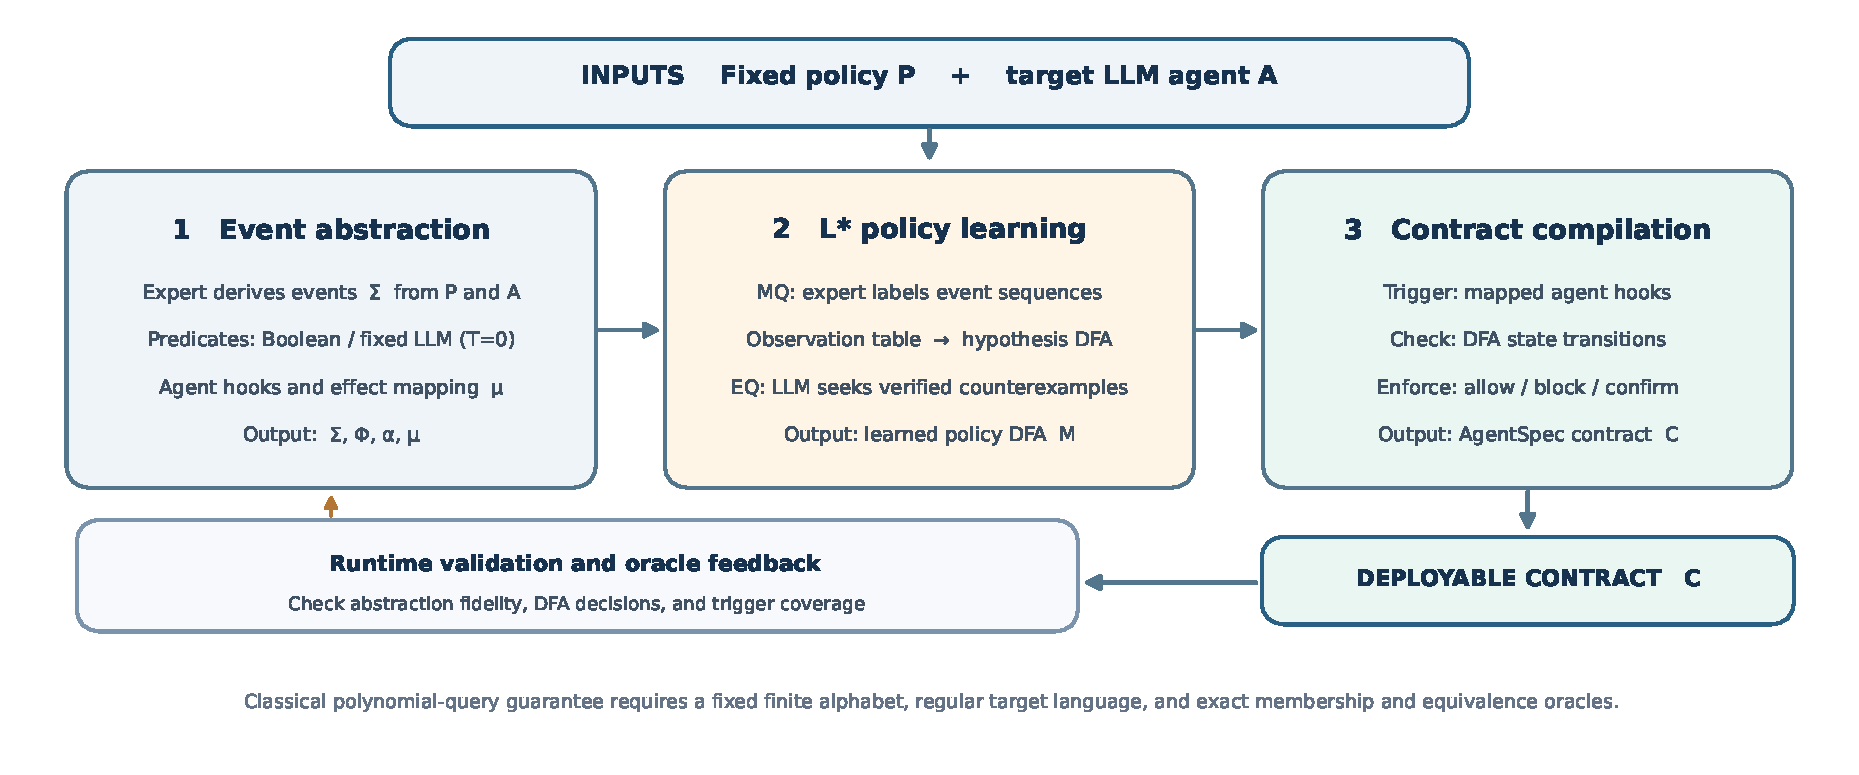
\includegraphics[width=0.94\textwidth,trim=0 52bp 0 0,clip]{figures/workflow_overview.pdf}
\caption{\system{} synthesizes an AgentSpec contract $C$ from an agent $A$, a policy $P$, and a labeled dataset $\mathcal{D}$. Agent-level instrumentation and expert-defined predicates produce ordered events over a fixed alphabet $\Sigma$. An $L^*$ learner answers membership queries from the dataset's labels where they apply and otherwise from an LLM that reads the policy, and refines its candidate DFAs with counterexamples: labeled trajectories on which the hypothesis is wrong. Event-to-hook mappings supply Trigger, the learned DFA supplies Check, and pre-effect mediation supplies Enforce. With correct labels and an LLM that is correct where the labels are silent, the learned DFA agrees with the whole dataset after at most $N-1$ counterexamples, and it is exact if the dataset is complete (Theorem~\ref{thm:exact}); exact enforcement additionally needs sufficient predicates and faithful interception (Corollary~\ref{cor:enforce}).}
\Description{Three phases: event abstraction from policy and instrumented agent, L-star learning with membership and counterexample queries, and compilation to AgentSpec trigger, check and enforce.}
\label{fig:workflow_overview}
\end{figure*}

\subsection{Phase 1: From Agent Execution to Event Streams}\label{sec:abstraction}
\paragraph{Selecting the observable events.}
A human or LLM expert examines $P$, the agent's tool schemas and workflows, and the available instrumentation points. It selects a finite alphabet $\Sigma$ of \emph{policy-relevant effects}, together with recognition predicates $\Phi$. A symbol is distinguished by the effect and policy-relevant context, not by the particular tool that produces it. The expert also specifies an event-to-hook mapping $\mu$, which identifies where each effect can be observed and, when consequential, intercepted before execution. The alphabet, predicates, and their implementations are fixed for a learning run; discovering that this abstraction is insufficient is reported as a limitation rather than silently changing the alphabet inside classical $L^*$.

\paragraph{Collecting and normalizing observations.}
Instrumentation at the agent's decision, tool-call, result, and state-update boundaries collects an ordered concrete trajectory $z=(o_1,\ldots,o_m)$, where each $o_i$ is an observation record. Records contain the proposed operation and its arguments, the correlated outcome, and the context needed to establish its actual policy-relevant effect. A proposal alone is not treated as a committed effect: failed or blocked calls do not emit the successful-effect symbol. If a tool invocation has several relevant effects, normalization yields separate, causally ordered records. LLM reasoning and other observations may contribute context without themselves producing an alphabet symbol. This normalization prevents, for instance, a failed public-link request from being confused with successful public disclosure.

\paragraph{Predicate-based event extraction.}
For each normalized record $o_i$, the recognizer evaluates $\Phi$ against $o_i$ and the relevant preceding context $h_i$. It emits either an event from $\Sigma$ or $\varepsilon$ (no policy-relevant event):
\[
 e_i=\operatorname{Recognize}_{\Phi}(o_i,h_i)
 \in\Sigma\cup\{\varepsilon\}.
\]
The context $h_i$ can include the current staging-slot contents, file sensitivity, effective link audience, and earlier tool outcomes, but is restricted to information available at the relevant observation point. The abstraction $\alpha$ concatenates the nonempty emissions in execution order:
\[
 \alpha(z)=e_1e_2\cdots e_m\in\Sigma^*,
\]
where $\varepsilon$ contributes no symbol. In the file-sharing example of Section~\ref{sec:motivating-example}, a successful confidential staging call emits $c$, replacement by a nonconfidential file emits $n$, and creation of a public link to the active staging slot emits $p$. Thus the executed sequence ``stage confidential, replace with normal, share publicly'' yields $\alpha(z)=cnp$ rather than $cp$. The replacement is a semantic effect established by the tool outcome, not guessed from the agent's stated intention.

\begin{table}[t]
\caption{Event extraction for the single-slot sharing agent. Only established effects emit events.}
\label{tab:event-extraction}
\centering\small
\begin{tabular}{p{0.47\columnwidth}p{0.39\columnwidth}}
\toprule
Observed outcome & Recognition and emission\\
\midrule
Stage confidential file successfully & Confidential payload $\rightarrow c$\\
Stage nonconfidential file successfully & Nonconfidential payload $\rightarrow n$\\
Create public link to active slot & Public audience $\rightarrow p$\\
Share request fails or is blocked & No committed effect $\rightarrow\varepsilon$\\
\bottomrule
\end{tabular}
\end{table}

Recognition predicates may be Boolean programs over structured fields or semantic classifiers implemented by a pinned LLM with a fixed prompt, output schema, and temperature zero. Repeated outputs for canonicalized inputs are cached. This improves repeatability, but neither temperature zero nor caching proves correct event classification. When the available evidence does not determine an event, the result is marked \texttt{unknown} and is not silently converted to $\varepsilon$. Before learning, sampled concrete traces are reviewed to check whether the abstraction preserves the policy distinctions needed for membership judgments. In particular, different concrete trajectories mapped to the same word must not have contradictory validated policy labels. A confirmed contradiction calls for expert review of the predicates or event meanings; abstraction refinement is outside the fixed-alphabet learning guarantee considered here.

\paragraph{Observations versus proposed effects.}
The same recognition rules support two execution phases. \emph{During learning}, $\alpha$ extracts events from successful effects observed in an isolated test environment. \emph{At deployment}, the trigger uses $\mu$ to recognize a proposed effect \emph{before commitment} and asks the monitor whether the corresponding event would be allowed. Only after the operation succeeds is the state transition committed. Proposed and observed effects must be reconciled; an unexpected or unclassifiable outcome requires a conservative fallback. This separation makes it possible to learn from real execution evidence while enforcing before an unsafe effect occurs.

\subsection{Phase 2: Active Learning of the Permissible Language}\label{sec:lstar}
\paragraph{Membership: labels first, then the policy.}
For a word $w\in\Sigma^*$, the ideal membership-query oracle answers $\operatorname{MQ}(w)=1$ iff $w\in L_G$, the ground-truth language of Section~\ref{sec:problem}. \system realizes it with two teachers. Before learning, the recognizer maps every trajectory of $\mathcal{D}$ to its word $\alpha(z)$, and the labels are entered into the answer cache under prefix closure: the word of a compliant trajectory and all its prefixes are members, and the word of a violating trajectory and all its extensions are non-members. Words determined both ways are collisions and are not entered. A membership query is then answered from the cache when the labels determine the word, so the labels always win. Only the remaining words reach an LLM with a pinned configuration, which reads the policy $P$, the event definitions and the sequence, and answers whether the sequence is acceptable. These are the words the data cannot settle: prefixes of violating trajectories, sequences that no trajectory contains, and words that no agent has realized yet. Here the policy is what generalizes the experience. If the LLM cannot decide, the query remains unresolved instead of receiving a fabricated label. Answers are cached with their provenance, label or LLM. For every word that the labels determine, \system also asks the LLM once, as a diagnostic: these answers are never used for learning, but their disagreements with the labels show where the policy does not summarize the experience. Theorem~\ref{thm:exact} assumes that the LLM is correct off the dataset (A3); Section~\ref{sec:rq2} measures how closely LLM judges meet that assumption.

\paragraph{Observation table and hypotheses.}
The $L^*$ learner~\cite{angluin1987learning} maintains a prefix set $S$, a set of distinguishing suffixes $E$, and a table $T$ of membership answers. Initially $S=E=\{\varepsilon\}$, where $\varepsilon$ is the empty word. For the one-event extensions $S\Sigma=\{sa\mid s\in S,a\in\Sigma\}$, the table contains
\[
 T(se)=\operatorname{MQ}(se),\quad
 s\in S\cup S\Sigma,\quad e\in E.
\]
The row $\operatorname{row}(s)=(T(se))_{e\in E}$ describes how history $s$ behaves under the tested continuations. The table is \emph{closed} when every row in $S\Sigma$ equals a row in $S$; it is \emph{consistent} when equal rows in $S$ remain equal after appending any alphabet event. A closure failure adds a representative history to $S$, whereas a consistency failure adds a distinguishing suffix to $E$. The learner obtains missing membership answers and repeats these steps until the table is closed and consistent. It then constructs a hypothesis DFA $\widehat M$ with one state per distinct row, transitions induced by one-event extensions, and accepting states given by membership of the corresponding histories.

For the alphabet $\Sigma=\{c,n,p\}$ of Section~\ref{sec:motivating-example}, the initial queries $\operatorname{MQ}(\varepsilon)$, $\operatorname{MQ}(c)$, $\operatorname{MQ}(n)$, and $\operatorname{MQ}(p)$ all return 1. Hence the first hypothesis accepts every word. The verified counterexample $cp$, with $\operatorname{MQ}(cp)=0$, exposes its error. Adding the suffix $p$ distinguishes the empty history from $c$, since $\operatorname{MQ}(p)=1$ but $\operatorname{MQ}(cp)=0$. Additional queries such as $\operatorname{MQ}(cnp)=1$ and $\operatorname{MQ}(ncp)=0$ establish how replacement staging affects future public sharing. Repeated table refinement can recover the three policy states in Figure~\ref{fig:sharing-dfa}; the developer does not provide their transition rules.

\paragraph{Equivalence checking against the dataset.}
An exact equivalence query asks whether the current DFA is correct and, if not, returns a counterexample word. No oracle answers it, and \system does not ask an LLM to: an LLM able to certify equivalence would make learning unnecessary (Section~\ref{sec:problem}). Instead, the labeled dataset answers it, so that every correction to the contract is backed by real feedback from the world. Each round replays the abstracted dataset through $\widehat M$, shortest words first, and returns the word $\alpha(z)$ of the first disagreement, a labeled trajectory $(z,y)$ with $\widehat M(\alpha(z))\neq y$, where $\widehat M(w)\in\{0,1\}$ is the hypothesis's acceptance decision. Since the membership teacher answers this word with its label, the counterexample is valid by construction; disagreements on collision words are reported and skipped. In the running example, labeled trajectories whose words are $cp$, $cnp$, and $ncp$ respectively challenge unsafe acceptance, erroneous over-restriction, and the effect of staging order. Because the label of a violating trajectory concerns the whole trajectory, its word may be longer than the shortest violating prefix; $L^*$'s counterexample processing adds the word's prefixes to the table, and membership queries locate the violation.

\paragraph{Learning loop and stopping condition.}
Each counterexample is returned to $L^*$, which refines its observation table and constructs another hypothesis. Learning stops when a hypothesis agrees with every labeled trajectory of $\mathcal{D}$ outside collisions, when an unresolved membership query suspends it, or when the budget is exhausted. The number of counterexamples never exceeds the number of distinct words in the dataset (Theorem~\ref{thm:exact}(a)). A returned DFA is \emph{dataset-consistent} (Theorem~\ref{thm:exact}(b)); it is exact on realizable words only if the dataset is complete (Theorem~\ref{thm:exact}(c)), which \system does not assume.

\paragraph{Query cost.}
Under (A2) and (A3), learning uses at most $O(|\Sigma|(B+1)N^2)$ membership queries, where $B$ is the length of the longest word in the dataset, and at most $N-1$ counterexamples, as in classical $L^*$~\cite{angluin1987learning}. Only the queries that the labels do not determine reach the LLM, plus one diagnostic query per distinct dataset word. Each round replays the dataset once, in time linear in its total length. These bounds count abstract queries. They do not bound LLM tokens or human review time, which Section~\ref{sec:eval} reports.

\subsection{Phase 3: DFA-to-AgentSpec Compilation}\label{sec:compile}
\paragraph{Trigger from concrete event mappings.}
The learned DFA determines which abstract event transitions may matter for the policy; $\mu$ maps those symbols back to concrete agent-tool and state-update hooks. The compiler instruments all events needed to maintain the DFA state, not only events that are immediately dangerous. Consequential calls whose proposed effects may enter a rejecting state must be intercepted before their effects commit. If multiple tools implement the same effect, all relevant implementations must be mapped. This is an agent-level integration contract, not an assumption of OS-wide interception.

\paragraph{Check from the learned DFA.}
For the learned hypothesis $\widehat M=(Q,\Sigma,\delta,q_0,F)$ defined in Section~\ref{sec:problem}, the monitor starts in state $q_0$. For a proposed event $e\in\Sigma$ at current state $q\in Q$, it computes $q'=\delta(q,e)$. For a prefix-closed hypothesis language, a transition to $q'\notin F$ is rejected before execution; otherwise, execution may proceed. The compiler checks this prefix-closure condition before claiming language-equivalent enforcement; a candidate that fails the check requires further learning or an explicitly reported conservative restriction. A successful effect commits $q'$, while a failed or blocked effect leaves the monitored policy state unchanged. Concurrent calls must be serialized or reconciled using a causally correct order. If the effect cannot be classified reliably before execution, the monitor follows a conservative fallback rather than allowing an unmonitored transition.

\paragraph{Enforce and validate.}
AgentSpec performs \texttt{ALLOW} or \texttt{BLOCK} according to the DFA check. A \texttt{CONFIRM} action or remediation is included only if a policy-defined procedure specifies its meaning and subsequent state effects; user confirmation alone is not assumed to turn a forbidden disclosure into a permissible one. The resulting contract is $C=\operatorname{Compile}(\widehat M,\alpha,\mu)$. Compilation is \emph{faithful} when the monitor accepts exactly the abstract words accepted by $\widehat M$ over the instrumented boundary. We test this property through transition-level differential replay and end-to-end interception, separately from the accuracy of the learned DFA and the adequacy of the abstraction. In particular, an accurate DFA cannot compensate for a missed trigger or an event classified after an irreversible effect.

% Evaluation (Section 5). All numbers come from results/REPORT.md and the logged runs in results/ of the
% SpecLearn artifact.
\section{Evaluation}
\label{sec:eval}\label{sec:evaluation}

This section reports a controlled study of \system{} on four sandboxed domains with reference oracles, which predates the dataset-based formulation of Section~\ref{sec:problem}. % TODO: add the real-world dataset evaluation (docs/EXPERIMENT_PLAN.md)
It answers four research questions:

\begin{description}
  \item[RQ1 (Exact membership).] When membership answers are exact, which equivalence checks let $L^*$ identify $L_G$,
  and how many expert labels does active learning need compared with passive and random-query learning?
  \item[RQ2 (Membership assumption).] How close do LLM membership judges come to the exact answers that assumption
  (A3) requires, and how do their errors propagate into the learned contracts?
  \item[RQ3 (Runtime fidelity).] Do the event abstraction and the compiled AgentSpec contracts enforce the
  learned model faithfully at runtime?
  \item[RQ4 (Safety and utility).] Do the synthesized contracts prevent policy violations of an LLM agent while
  preserving its legitimate tasks, compared with expert-written rules and direct LLM synthesis?
\end{description}

% -------------------------------------------------------------------------------------
\subsection{Experimental Setup}
\label{sec:setup}

\paragraph{Agent domains.}
We built four instrumented agent domains (Table~\ref{tab:domains}). Each provides the inputs of \system{}: a fixed
natural-language policy $P$, a tool API, a deterministic sandbox, and an expert-written event abstraction
$(\Sigma,\Phi,\mu)$ with Boolean recognition predicates over visible fields. Each domain also has a reference DFA and an independent concrete policy checker. The checker inspects the ground-truth
effects of tool calls and never uses $\Sigma$. Together they serve as the ground truth (A5) and as the reference for the
metrics; in the runs below, ground-truth labels are taken from the reference DFA, which agrees with the checker within
the bounds stated next. \dom{DocShare} is the running example of Section~\ref{sec:motivating-example}.

We checked policy sufficiency (Section~\ref{sec:problem}) within bounds: the checker agrees with the reference DFA on the canonical concretization of
every abstract word up to length 4--5 and on every concrete action sequence of length at most 3.

The domains contain the difficulties the method must handle:
\begin{itemize}
  \item unlabeled files (\dom{DocShare});
  \item a multi-effect tool and an outcome-dependent approval step (\dom{Payments});
  \item unannotated SQL migrations (\dom{DevOps});
  \item synonym field names (\dom{DataExport});
  \item alias tools that produce the same effect (three domains).
\end{itemize}
Each domain has 12--13 held-out tasks: 6--7 benign and 6 unsafe, 49 in total. The unsafe tasks ask for an action that
would violate $P$. Each domain also has 8 training tasks, used only by passive inference.

\begin{table}[t]
  \caption{Agent domains. $|\Sigma|$: events; $|Q|$: states of the minimal reference DFA; tasks: held-out
  benign/unsafe tasks.}
  \label{tab:domains}
  \small
  \setlength{\tabcolsep}{3pt}
  \begin{tabular}{@{}p{1.55cm}p{4.0cm}ccc@{}}
    \toprule
    Domain & Policy $P$ (abridged) & $|\Sigma|$ & $|Q|$ & Tasks \\
    \midrule
    \dom{DocShare} & Confidential documents must not become accessible to unauthorized parties. & 3 & 3 & 6/6 \\
    \dom{Payments} & Payments above \$1{,}000 need a manager's approval; an approval covers one execution and is voided by any change. & 4 & 4 & 6/6 \\
    \dom{DevOps} & Deploy only if tests passed after the latest change; a destructive migration needs a fresh backup. & 6 & 5 & 7/6 \\
    \dom{DataExport} & No personal data to external recipients unless anonymized; at most two external reports. & 5 & 6 & 6/6 \\
    \bottomrule
  \end{tabular}
\end{table}

\paragraph{Target agent and LLMs.}
The target agent $A$ is a JSON tool-calling agent built on Qwen3-30B-A3B. It is \emph{not} told the policy, so the
contract has to constrain it independently of its own decisions.

All LLMs are open-weight models served locally with MLX on an Apple M3 Ultra (96\,GB). They use greedy decoding
(temperature 0) and fixed prompts. The roles are:
\begin{itemize}
  \item \emph{Membership judge:} Qwen3-30B-A3B. It is shown the word's canonical execution in the sandbox, a scripted
  concretization rather than an agent run, and uses a step-wise prompt. Its reasoning mode is used only to escalate unresolved queries.
  \item \emph{Scenario writer for agent-realized tests:} Qwen3-14B. Using a separate model lets judge errors
  and tester errors be told apart.
  \item \emph{LLM event recognizer:} Qwen3-30B-A3B.
\end{itemize}
\systemR{} denotes the same configuration with the judge's reasoning mode always enabled.

\paragraph{Implementation.}
\system{} is 5.5k lines of Python.
\begin{itemize}
  \item \emph{Learner.} $L^*$ with Angluin's counterexample processing.
  \item \emph{Membership service.} It caches labels with their provenance and infers the labels implied by prefix
  closure~\cite{hungar2003domain}. It escalates unresolved queries, and it suspends learning if no oracle resolves a query rather than invent a
  label.
  \item \emph{Equivalence check.} The implementation predates the ground-truth formulation of Section~\ref{sec:lstar}:
  it labels equivalence tests with the active membership oracle. With exact oracles these labels are ground truth;
  with an LLM judge they are not. It builds its tests online rather than replaying a fixed dataset. Each equivalence
  query first runs 6 agent-realized tests: the scenario writer turns a target word into a task, the agent executes it
  in a fresh sandbox, and the realized word $\alpha(z)$ is labeled. Up to 120 hypothetical tests follow, from
  hypothesis-guided selection: the access words of the hypothesis states, extended by $\Sigma^{\le 2}$ and the
  distinguishing suffixes $E$, prioritized by transitions that enter or lie next to the rejecting region, then by
  untested event pairs. They predate the use of a fixed labeled dataset.
  \item \emph{Budget.} Runs labeled by an LLM are capped at 400 labels and 12 equivalence queries.
  \item \emph{Compiler.} It emits one AgentSpec rule per rejecting DFA transition, with \texttt{event\_$e$} and
  \texttt{state\_$q$} predicates, and enforces before execution (\texttt{llm\_self\_examine}: the call is not executed, and the agent may continue).
  \item \emph{Runtime recognition.} The runtime uses a hybrid recognizer: Boolean predicates first, and the LLM only
  when they abstain.
\end{itemize}

\paragraph{Compared conditions.}
We compare six conditions:
\begin{enumerate}
  \item \emph{Expert-written AgentSpec rules}, in two variants over a generic past-time predicate library with the
  operators \texttt{ever}, \texttt{last}, \texttt{since} and \texttt{count}. The \emph{careful} rules are correct by construction.
  The \emph{naive} rules contain plausible omissions, such as the naive rules discussed in Section~\ref{sec:motivating-example}.
  \item \emph{LLM direct synthesis.} From $P$, $\Sigma$ and the tool schemas, the LLM writes either a DFA over $\Sigma$
  or AgentSpec rules over the same predicate library, in one call. We report Qwen3-30B-A3B with reasoning, the
  strongest of seven model configurations.
  \item \emph{Passive inference}: RPNI~\cite{oncina1992rpni} on the labeled prefixes of the agent's executions of the training tasks.
  \item \emph{Random-query learning}: RPNI on randomly chosen words, labeled at the label budget of the matched active
  learner.
  \item \emph{$L^*$ with exact oracles}, backed by the reference DFA.
  \item \emph{\system{}} and \emph{\systemR{}} with practical experts. The LLM judge labels both the membership
  queries and the equivalence tests. Section~\ref{sec:problem} argues against this for equivalence; we report it as
  measured; the split teacher of Section~\ref{sec:lstar}, with labels first, remains to be evaluated.
\end{enumerate}

\paragraph{Metrics.}
\begin{itemize}
  \item \emph{Language level} (Definition~\ref{def:policy-language}). The unsafe-permission rate (UP) is
  $|(L(C)\setminus L_G)\cap\Sigma^{\le\ell}|/|\Sigma^{\le\ell}\setminus L_G|$, and the over-restriction rate (OR) is
  $|(L_G\setminus L(C))\cap\Sigma^{\le\ell}|/|L_G\cap\Sigma^{\le\ell}|$. Unless stated otherwise, $\ell=6$ ($\ell=5$ for
  \dom{DevOps}). Each word is replayed through the contract's monitor, so DFA-based and rule-based contracts are measured
  identically. The rates depend on $\ell$: \systemR{}'s over-restriction on \dom{DevOps} is 5.2\% at $\ell=5$ but
  19.0\% at $\ell=10$.
  \item \emph{Online.} The agent runs every held-out task with the contract in the loop. We count the unsafe tasks in
  which a violation is committed and the benign tasks completed without violation.
  \item \emph{Cost.} Expert labels and LLM tokens.
\end{itemize}

\paragraph{Reproducibility.}
Randomness is seeded. Every LLM response is cached under a hash of the model revision, prompt and decoding parameters.
Re-running all experiments from the cache reproduced all 191 result files exactly.
% TODO: anonymized artifact link

% -------------------------------------------------------------------------------------
\subsection{RQ1: Learning with Exact Membership}
\label{sec:rq1}

\paragraph{Controlled targets.}
We first validated the learner on 200 random minimal prefix-closed DFAs with 4 to 64 states and 2 to 16 events,
10 per combination, each learned under 15 configurations (3{,}000 runs). We used an exact membership oracle, an exact equivalence oracle that returns the
shortest counterexample or one padded to a length of at least 10, 25, 50 or 100, and three counterexample-processing strategies: Angluin's~\cite{angluin1987learning}, Maler--Pnueli's~\cite{maler1995learnability},
and Rivest--Schapire's~\cite{rivest1993inference}.

\begin{itemize}
  \item $L^*$ recovered the minimal target in all 3{,}000 runs and never needed more than $N-1$ counterexamples.
  \item The number of distinct membership queries grew roughly as $N^{1.6}$ and as $|\Sigma|^{1.1}$. It stayed below
  49\% (median 8\%) of the classical bound $O(|\Sigma|(B+1)N^2)$.
  \item Long counterexamples inflate the queries of Angluin's strategy ($\times 4.9$ at $B=100$, $N=32$, $|\Sigma|=4$)
  and of Maler--Pnueli's ($\times 7.9$), but not those of Rivest--Schapire's (1{,}606 vs.\ 1{,}685).
  \item On \dom{DocShare} the observation table reproduces the walk-through of Section~\ref{sec:motivating-example}. The first hypothesis has one
  state; the verified counterexample \texttt{c\,p} adds suffix \texttt{p} through a consistency fix; MQ(\texttt{c\,n\,p})
  $=1$ separates \texttt{c} from \texttt{c\,n}; the result is the three-state DFA of Figure~\ref{fig:sharing-dfa}.
\end{itemize}

\paragraph{Domains.}
Table~\ref{tab:rq1} shows the label cost. With exact labels, the equivalence tests are ground-truth-labeled: agent-realized tests
form an online corpus of labeled agent trajectories, and the guided suite adds labeled abstract words. Neither is
checked for completeness. % TODO: replace with the real-world dataset experiments of docs/EXPERIMENT_PLAN.md
\begin{itemize}
  \item With exact equivalence queries, $L^*$ recovers all four reference DFAs with 11--111 labels.
  \item Agent-realized tests alone, with exact labels and 10 tests per equivalence query (instead of the default 6), recover \dom{DocShare} and
  \dom{DevOps} but stop prematurely on \dom{Payments} and \dom{DataExport}, leaving 4.3\% and 17.4\% unsafe
  permissions. The missing distinctions need long sequences (approval consumption, \texttt{ml\,ap\,ex\,ex}; a third
  external send). Every disagreement this corpus exposed was genuine, but it ran out of disagreements before the hypothesis was correct:
  the corpus was incomplete.
  \item The hypothesis-guided suite recovers all four, at 27--311 labels. Its final query spends its budget without finding
  a disagreement, so the result is only consistent with its tests; nothing certifies it.
  \item Random-word equivalence testing recovers \dom{DataExport} in only 4 of 10 seeds.
  \item At the same label budgets, random-query learning recovers only \dom{DocShare} (0 of 10 seeds elsewhere, up to
  7.1\% UP).
  \item Passive inference from the training traces recovers only \dom{DocShare} (up to 42\% UP elsewhere).
\end{itemize}

We also swept the equivalence budget (exact labels, 20 seeds). Hypothesis-guided testing removes premature stops at 40 labels
per equivalence query on \dom{Payments} and \dom{DevOps}, and at 160 on \dom{DataExport}. At 160 labels, random
testing still stops prematurely in 5\% (\dom{Payments}) and 50\% (\dom{DataExport}) of runs. Random testing is
competitive only where violations are dense: on \dom{DevOps} with 10 labels it stops prematurely in 10\% of runs, against
80\% for hypothesis-guided testing.

\begin{table}[t]
  \caption{Learning with exact labels. $L^*$ and Guided EQ (hypothesis-guided bounded testing): expert labels until
  termination (both learned the exact DFA). Random EQ and Random query: seeds (of 10) that learned $L_G$ exactly; Random
  query uses the Guided-EQ label budget. Passive: labels used and whether the result is exact.}
  \label{tab:rq1}
  \small
  \setlength{\tabcolsep}{3pt}
  \begin{tabular}{@{}lccccc@{}}
    \toprule
    Domain & $L^*$ & Guided & Random & Random & Passive \\
    & (exact EQ) & EQ & EQ & query & \\
    \midrule
    \dom{DocShare}   & 11  & 27  & 10/10 & 10/10 & 10, yes \\
    \dom{Payments}     & 36  & 103 & 10/10 & 0/10  & 14, no \\
    \dom{DevOps}       & 73  & 195 & 10/10 & 0/10  & 14, no \\
    \dom{DataExport} & 111 & 311 & 4/10  & 0/10  & 10, no \\
    \bottomrule
  \end{tabular}
\end{table}

\answerbox{RQ1}{With exact membership and equivalence oracles, $L^*$ identifies every target, as classical $L^*$
guarantees: all 3{,}000 synthetic runs (200 targets) and all four domain policies. With ground-truth labels
but no completeness, agent-realized trajectories alone stop early on two of four domains, and the budget-capped
hypothesis-guided suite recovers all four without a certificate. Learning against a fixed real-world labeled dataset is not yet evaluated.
Random-query learning at the same label budget and passive learning from the training traces each learn only one of
the four contracts.}

% -------------------------------------------------------------------------------------
\subsection{RQ2: The Membership Assumption}
\label{sec:rq2}

\paragraph{Membership judges.}
We measured judges on 178 independently labeled words (Table~\ref{tab:judges}). The set contains all or sampled words of
length at most 2, plus 24 longer words per domain balanced over three categories: permitted, violating at the last event,
and violating earlier.

\begin{itemize}
  \item The primary judge is 87.6\% accurate (100/87/81/85\% per domain).
  \item Abstract evidence gives the same accuracy as grounded evidence but shifts the errors: more over-rejection
  (19.2\% vs.\ 13.5\%) and fewer unsafe acceptances (1.4\% vs.\ 8.1\%).
  \item A direct (non-step-wise) prompt or a paraphrased yes/no prompt costs 7 points.
  \item With reasoning enabled, the judge labels all 178 words correctly, at about $1.8\times$ the tokens.
  \item Verdicts are deterministic: 48 judgments regenerated without the cache were all reproduced. They are not robust
  to wording: the primary judge changes its verdict on 15--19\% of words under a paraphrased prompt, renamed event
  symbols or abstract evidence.
  \item Other models fail in opposite directions. Llama-3.1-8B accepts 69\% of prohibited words; Qwen3-4B and Qwen3-14B
  reject about half of the permitted ones.
\end{itemize}

\begin{table}[t]
  \caption{LLM membership judges on 178 labeled words. Acc.: accuracy; UA: prohibited words judged permitted; OR:
  permitted words judged violating.}
  \label{tab:judges}
  \small
  \setlength{\tabcolsep}{4pt}
  \begin{tabular}{@{}lrrr@{}}
    \toprule
    Judge configuration & Acc. & UA & OR \\
    \midrule
    Qwen3-30B, grounded, step-wise (primary) & 87.6 & 8.1 & 13.5 \\
    \quad abstract evidence                  & 87.6 & 1.4 & 19.2 \\
    \quad direct prompt                      & 80.9 & 10.8 & 19.2 \\
    \quad paraphrased (yes/no) prompt        & 80.3 & 9.5 & 25.0 \\
    \quad reasoning enabled                  & \textbf{100.0} & 0.0 & 0.0 \\
    Qwen3-32B, grounded, direct              & 91.0 & 10.8 & 7.7 \\
    Mistral-Small-24B, grounded, direct      & 86.0 & 1.4 & 23.1 \\
    Llama-3.1-8B, grounded, direct           & 70.8 & 68.9 & 1.0 \\
    Qwen3-4B, grounded, direct               & 68.5 & 10.8 & 46.2 \\
    Qwen3-14B, grounded, direct              & 68.0 & 0.0 & 51.9 \\
    \bottomrule
  \end{tabular}
\end{table}

\paragraph{Sensitivity to label errors.}
With simulated persistent noise, each word's label is flipped with probability $\rho$ (20 seeds, hypothesis-guided
equivalence testing). Exact recovery falls from 100\% to 5--75\% at $\rho=1\%$, and to 0--15\% at $\rho=5\%$. At
$\rho=5\%$ the contracts over-restrict 23--29\% of permitted words and permit 5--9\% of prohibited ones (words up to
length 8).

\paragraph{Learning with LLM judges.}
Table~\ref{tab:rq2} shows the learned contracts. Both configurations learn \dom{DocShare} exactly from 29 labels.

Without reasoning, the judge mislabels 19--36\% of the queries $L^*$ asks in the other domains. The errors are mostly
over-cautious ``violation'' verdicts, for instance treating setting a large draft payment as paying it, plus lost counts
on long sequences. $L^*$ exhausts its budget with 9--17-state monitors that over-restrict 15--61\% of permitted words.

With reasoning, the error rate drops to 0.3--6\%. The \dom{Payments} contract is practically exact (one over-restricted
word out of 3{,}910), and \dom{DevOps} reaches 3.3\% UP and 5.2\% OR. Three effects remain:
\begin{enumerate}
  \item \emph{One wrong label can prevent convergence.} On \dom{Payments}, a single wrong label kept $L^*$ from
  converging: it spent the remaining budget adding states to explain it (10 states instead of 4). Because the same
  judge labeled the equivalence tests, they could not expose the error; a label for that word would have overridden it.
  \item \emph{Balanced word sets overstate accuracy.} The judge that was perfect on the balanced word set errs on
  3.5--6\% of the learner's queries, which are long and probe the policy boundary. On \dom{DataExport} it consistently
  judged reading personal data and then sending it to an internal recipient to be a violation.
  \item \emph{Long queries can exhaust the reasoning budget.} Learning on \dom{DataExport} was suspended when the judge
  used up its reasoning budget on a 10-event query without reaching a verdict.
\end{enumerate}

\begin{table}[t]
  \caption{Contracts learned with LLM judges. States: learned/reference. Wrong: mislabeled queries / queries judged. UP/OR (\%): language level,
  all words up to length 6 (5 for \dom{DevOps}). $^\dagger$label budget exhausted; $^\ddagger$suspended on an unresolved query.}
  \label{tab:rq2}
  \small
  \setlength{\tabcolsep}{3pt}
  \begin{tabular}{@{}lcrr@{\hspace{8pt}}crr@{}}
    \toprule
    & \multicolumn{3}{c}{\system{}} & \multicolumn{3}{c}{\systemR{}} \\
    \cmidrule(r){2-4}\cmidrule(l){5-7}
    Domain & States & Wrong & UP/OR & States & Wrong & UP/OR \\
    \midrule
    \dom{DocShare}   & 3/3 & 0/29 & 0.0/0.0 & 3/3 & 0/29 & 0.0/0.0 \\
    \dom{Payments}     & 13/4$^\dagger$ & 144/400 & 17.2/60.2 & 10/4$^\dagger$ & 1/399 & 0.0/0.03 \\
    \dom{DevOps}       & 17/5$^\dagger$ & 94/395  & 4.7/60.5  & 13/5$^\dagger$ & 14/399 & 3.3/5.2 \\
    \dom{DataExport} & 9/6$^\dagger$  & 74/399  & 7.4/15.2  & 11/6$^\ddagger$ & 16/266 & 17.3/10.2 \\
    \bottomrule
  \end{tabular}
\end{table}

\paragraph{Agent-realized tests.}
The scenario writer and the agent reproduced the target word exactly in 53--94\% of tests. Within \system{},
agent-realized tests produced 1--3 verified counterexamples per domain. Used alone with exact labels, they stop early
on two domains (Section~\ref{sec:rq1}).

\answerbox{RQ2}{Current LLM judges do not meet assumption (A3), and $L^*$ amplifies even a few wrong labels into
oversized, over-restrictive monitors. A non-reasoning judge (88\% accurate) yields one exact contract out of four; the same model
with reasoning yields one exact and one practically exact contract. Judge accuracy must be measured on the learner's own
queries, which are harder than balanced samples.}

\begin{table*}[t]
  \caption{Safety and utility. Language level: unsafe-permission / over-restriction rate (\%) over all words up to length
  6 (5 for \dom{DevOps}). Online: unsafe held-out tasks with a committed violation, and benign tasks completed without
  violation. LLM direct synthesis uses Qwen3-30B-A3B with reasoning. $^\dagger$Labeled by the same LLM judge as
  \system{}: random-query learning at \system{}'s label budget, passive inference on the labeled training traces. Online runs were performed for the listed conditions only.}
  \label{tab:rq4}
  \small
  \begin{tabular}{@{}lccccrr@{}}
    \toprule
    & \multicolumn{4}{c}{Language level: UP / OR (\%)} & \multicolumn{2}{c}{Online} \\
    \cmidrule(r){2-5}\cmidrule(l){6-7}
    Condition & \dom{DocShare} & \dom{Payments} & \dom{DevOps} & \dom{DataExport} & Violations & Benign done \\
    \midrule
    No contract                        & 100 / 0.0 & 100 / 0.0 & 100 / 0.0 & 100 / 0.0 & 21/24 & 24/25 \\
    Expert rules, careful              & 0.0 / 0.0 & 0.0 / 0.0 & 0.0 / 0.0 & 0.0 / 0.0 & 0/24 & 23/25 \\
    Expert rules, naive                & 0.0 / 26.4 & 40.4 / 0.0 & 14.6 / 0.0 & 16.3 / 8.8 & 7/24 & 19/25 \\
    LLM direct synthesis, DFA          & 0.0 / 0.0 & 4.3 / 0.0 & 0.0 / 4.0 & 0.0 / 0.0 & 2/24 & 22/25 \\
    LLM direct synthesis, rules        & 0.0 / 0.0 & 4.3 / 0.0 & 28.5 / 28.7 & 0.0 / 0.0 & 4/24 & 23/25 \\
    Passive inference (RPNI)$^\dagger$ & 0.0 / 0.0 & 10.6 / 34.3 & 14.0 / 35.3 & 42.4 / 27.9 & 3/24 & 20/25 \\
    Random-query learning$^\dagger$    & 0.0 / 0.0 & 5.7 / 43.7 & 6.7 / 44.7 & 25.7 / 11.1 & 1/24 & 21/25 \\
    $L^*$ with exact oracles           & 0.0 / 0.0 & 0.0 / 0.0 & 0.0 / 0.0 & 0.0 / 0.0 & 0/24 & 22/25 \\
    \midrule
    \system{}                       & 0.0 / 0.0 & 17.2 / 60.2 & 4.7 / 60.5 & 7.4 / 15.2 & 3/24 & 19/25 \\
    \systemR{}                      & 0.0 / 0.0 & 0.0 / 0.03 & 3.3 / 5.2 & 17.3 / 10.2 & 1/24 & 22/25 \\
    \bottomrule
  \end{tabular}
\end{table*}

% -------------------------------------------------------------------------------------
\subsection{RQ3: Runtime Fidelity}
\label{sec:rq3}

\paragraph{Event recognition.}
Table~\ref{tab:recognizers} summarizes recognition on the scripted corpus.
\begin{itemize}
  \item \emph{Boolean predicates} never misclassify an effect, but they abstain on up to 40\% of effects, such as
  unlabeled files, unannotated SQL and synonym field names. The conservative monitor turns abstentions into
  over-blocking.
  \item \emph{LLM predicates} never abstain, but misclassify 20--32\% of effects. With the \emph{reference} DFA, this
  alone causes 31 false permissions.
  \item \emph{Hybrid recognition} is 93--100\% accurate with zero false permissions. Its residual over-blocks come from
  the LLM misreading an unannotated \texttt{UPDATE} migration or an unlabeled public file.
\end{itemize}

\begin{table}[t]
  \caption{Event recognition on 300 scripted executions per domain: accuracy (abstentions) in \%, and the false
  permissions (FP) and over-restrictions (OR) that recognition alone causes under the reference DFA, summed over domains.}
  \label{tab:recognizers}
  \small
  \setlength{\tabcolsep}{3.5pt}
  \begin{tabular}{@{}lccccrr@{}}
    \toprule
    Recognizer & \dom{Doc} & \dom{Pay} & \dom{Dev} & \dom{Data} & FP & OR \\
    \midrule
    Boolean & 60 (40) & 100 (0) & 87 (13) & 98 (2) & 0 & 102 \\
    LLM     & 80 (0)  & 68 (0)  & 73 (0)  & 78 (0) & 31 & 136 \\
    Hybrid  & 98 (0)  & 100 (0) & 93 (0)  & 100 (0) & 0 & 51 \\
    \bottomrule
  \end{tabular}
\end{table}

\paragraph{Policy sufficiency.}
To find collisions, we realized every abstract word up to length 3--4 through all concrete call sequences of the sandbox
and labeled each realization with the independent checker.
\begin{itemize}
  \item With exact Boolean recognition, the expert alphabet produces no contradictory word in any domain (873 realizable
  words).
  \item With the hybrid recognizer used at runtime, LLM misreadings make 24.2\% (\dom{DocShare}) and 16.7\%
  (\dom{DevOps}) of the realizable words contradictory: recognition errors break sufficiency (A1) just as a coarse
  alphabet does.
  \item A naive ``event = tool name'' alphabet has 19--63\% contradictory words.
  \item Vocabularies derived by two LLMs (ablation~i) drop the distinctions that matter: file sensitivity, the payment
  threshold and approval semantics, and destructiveness. They are contradictory on up to 69\% of words (\dom{DevOps}).
  Contracts learned over them with an exact grounded oracle give 7--100\% false permissions.
\end{itemize}

\paragraph{Compilation.}
All 142 DFA-based contracts produced in the evaluation agree with the DFA they were compiled from on every reachable
transition (4{,}059 decision and state-update checks) and on all 1.37\,M words up to the length bound. Executed end to end
on concrete calls, including alias tools, the reference and exact-$L^*$ contracts agree with their DFA on 100\% of
decisions.

One contract deviates: the noisy \system{} contract for \dom{DevOps}, at 89\%. The cause is semantic, not the
compiler. Its DFA rejects one outcome of \texttt{run\_tests}, and the outcome is unknown before execution, so the
pre-effect check must block the call.

\paragraph{Instrumentation and timing.}
Leaving one alias tool out of $\mu$ lowers trigger interception recall from 100\% to 18--94\%. Online, the agent then
bypassed the contract through the unmapped tool in 2--3 of the 6 unsafe episodes per domain (33--50\% violations
instead of 0\%). Used as a post-effect detector, the same contract flags violations but prevents none: 67--100\% of
unsafe episodes violate. A monitor check takes 1.5--2.1\,$\mu$s with Boolean recognition.

\answerbox{RQ3}{Compilation is faithful for all 142 contracts. The weak points lie at the boundary between the model and
the agent:
\begin{itemize}
  \item recognizers must abstain rather than guess, and hybrid recognition eliminates the false permissions;
  \item the alphabet must preserve the policy's distinctions, which the expert alphabet does and LLM-derived ones do
  not, and recognition must not merge them, which the deployed hybrid recognizer does on 17--24\% of words in two
  domains;
  \item every tool that produces a relevant effect must be hooked;
  \item enforcement must happen before the effect commits.
\end{itemize}}

% -------------------------------------------------------------------------------------
\subsection{RQ4: Safety and Utility}
\label{sec:rq4}

Table~\ref{tab:rq4} compares all conditions.

\paragraph{Baselines.}
\begin{itemize}
  \item Without a contract, the agent commits a violation in 21 of the 24 unsafe held-out tasks.
  \item Contracts learned from exact labels and the careful expert rules are exact in all four domains. They prevent
  every violation online while completing 22--23 of the 25 benign tasks. The two benign failures in \dom{DocShare} are
  shared by all contracts: the hybrid recognizer classifies an unlabeled public file as confidential.
  \item The naive expert rules miss approval consumption, the test-after-change requirement and the egress limit
  (15--40\% UP), giving violations in 7 tasks.
  \item Direct synthesis with reasoning is exact on \dom{DocShare} and \dom{DataExport}. It misses approval consumption
  on \dom{Payments} (4.3\% UP), and its rules leave 28.5\% UP on \dom{DevOps}, which leads to 2 (DFA) and 4 (rules)
  online violations. Without reasoning, the same model produces monitors with up to 100\% UP or 94\% OR.
\end{itemize}

\paragraph{\system{}.}
With the non-reasoning judge, \system{} lets 3 violations through and completes 19 benign tasks. \systemR{} lets 1
violation through and completes 22 benign tasks, the same utility as the exact contracts.

\paragraph{Cost.}
Exact $L^*$ needs 11--111 labels (27--311 with bounded equivalence testing). With an LLM judge, \system{} spent 29
labels on \dom{DocShare} and its full 400-label budget elsewhere; \systemR{} was suspended after 266 labels on
\dom{DataExport}. That is 45k--480k LLM tokens per contract without
reasoning and 56k--972k with reasoning. Direct synthesis takes one call of 1.6k--8.1k tokens.


\answerbox{RQ4}{Contracts learned with exact oracles prevent every violation, as the careful expert rules do, and
complete 22 of 25 benign tasks (the careful rules complete 23), without any manually written rule. With practical LLM
judges, \systemR{} lets 1 of 24 unsafe tasks through and completes 22 benign tasks. Online, this is on par with direct
LLM synthesis (2--4 of 24) and random-query learning with the same judge (1 of 24): 24 tasks are too few to separate
them, and at the language level direct DFA synthesis is more accurate than \systemR{} on \dom{DevOps} and
\dom{DataExport}. All are well ahead of naive expert rules (7 of 24). \systemR{} costs up to about 1M tokens per
contract.}

% -------------------------------------------------------------------------------------
\subsection{Threats to Validity}
\label{sec:threats}

\paragraph{Internal.}
We wrote the domains, the reference DFAs, the concrete checkers, the expert abstraction and both expert rule sets. The
careful rules are correct by construction; the naive rules are illustrative and do not estimate how often developers
make such mistakes.

\paragraph{External.}
The four domains are small sandboxes ($|\Sigma|\le 6$, at most 6 states). All LLMs are local open-weight models rather
than frontier models. No human experts took part: simulated label noise stands in for them. AgentSpec contracts run on a
re-implemented runtime with AgentSpec's rule syntax and semantics.

\paragraph{Construct.}
Language-level rates weight all words up to the length bound equally, while online measures weight the behaviors the
agent actually produces; we report both. With 49 held-out tasks, online rates are uncertain. LLM-labeled runs are capped at
400 labels, so runs that do not converge are reported with their last hypothesis.

\section{Related Work and Positioning}
\paragraph{Runtime safety contracts for agents.}
AgentSpec provides the customizable trigger--check--enforce interface into which we compile the learned monitor~\cite{wang2026agentspec}. RvLLM motivates natural-language safety predicates grounded in execution context~\cite{zhang2025rvllm}, while Agent Behavioral Contracts studies runtime behavioral constraints~\cite{bhardwaj2026abc}. ShieldAgent verifies agent actions against safety policies extracted from documents~\cite{chen2025shieldagent}, Progent enforces programmable privilege policies on tool calls~\cite{shi2025progent}, and CaMeL separates control and data flow to defeat prompt injection by design~\cite{debenedetti2025camel}. Our monitors are security automata in Schneider's sense~\cite{schneider2000enforceable}: they enforce safety properties by blocking, a subclass of what edit automata can enforce~\cite{ligatti2005edit}, and they resemble shields that block the unsafe actions of a learning agent~\cite{alshiekh2018shielding}. Our contribution is a pipeline for obtaining an executable policy check from active learning rather than requiring the developer to write every behavioral condition.

\paragraph{Active automata learning.}
Angluin's $L^*$ constructs a DFA using a closed and consistent observation table, membership queries, and equivalence counterexamples~\cite{angluin1987learning}. We use its observation table, closure and consistency tests, and counterexample loop unchanged, rather than treating distinguishing queries as a heuristic. In practice, equivalence oracles are approximated by conformance testing: the W-method is complete for systems with a known bound on their number of states~\cite{chow1978testing,vasilevskii1973failure}, black-box checking combines it with $L^*$~\cite{peled1999blackbox}, and random sampling yields probably approximately correct identification~\cite{angluin1988queries}. Without an equivalence oracle, exact identification needs exponentially many membership queries in the worst case~\cite{angluin1981note}. \system approximates the equivalence oracle with trajectories that carry ground-truth labels, so that the certificate does not rest on the membership expert, and it uses an LLM only for membership, never to judge equivalence. Inferring labels by prefix closure follows domain-specific optimizations of automata learning~\cite{hungar2003domain}. Learning with erroneous membership answers~\cite{sakakibara1991noise,angluin1997malicious} relaxes our exact-membership assumption, and teachers that may answer ``don't know''~\cite{grinchtein2006learning} correspond to our unresolved queries. Mappers~\cite{aarts2015mappers} and automated alphabet refinement~\cite{howar2011alphabet} motivate revisiting event definitions when abstractly identical traces receive conflicting policy labels. The research challenges are interfacing $L^*$ with natural-language policies, event extraction from instrumented agent behavior, practical expert oracles, and faithful runtime compilation.

\paragraph{Learning specifications with language models.}
L$^*$LM uses a language model as a natural-language oracle when learning automata from examples~\cite{vazquez2024lstarlm}, and nl2spec translates natural language into temporal logic with an LLM in the loop~\cite{cosler2023nl2spec}. Extracting automata from neural networks with $L^*$~\cite{weiss2018extracting} faces a related gap between a non-symbolic teacher and an automaton. \system differs in its target, an enforced runtime contract for a given agent, and in grounding membership questions in sandbox executions of that agent's tools.

\paragraph{Policy and rule synthesis.}
AutoSpec investigates programmable rule synthesis from annotated examples~\cite{ma2026autospec}, while PolicyBank integrates corrected policy knowledge into an agent's memory~\cite{choi2026policybank}. SEVerA evolves agent programs subject to supplied safety constraints~\cite{banerjee2026severa}. These systems differ in the learned artifact and its enforcement boundary. \system learns an abstract permissible-behavior DFA and compiles it into an independent AgentSpec runtime contract for a given target agent. Incremental maintenance following agent evolution, including cases illustrated by Misevolution~\cite{shao2025misevolve}, remains complementary future work rather than an evaluated claim.

\section{Limitations}\label{sec:limitations}
\paragraph{Scope and finite-state assumption.}
This work addresses synthesis for a fixed target LLM agent, for which we assume that the event predicates are sufficient (A1). An evolving agent can break this assumption: new tools or behaviors can produce trajectories that the predicates map to the same word despite different policy judgments. The abstraction must then be refined and the contract re-learned, which we leave to future work on contract evolution. A high-level policy may also require unbounded identities, counters, data values, or obligations that no regular language over a practical finite alphabet captures (A2). We focus on prefix-closed safety properties, where a prohibited effect has an observable bad prefix and pre-effect interception is meaningful.

\paragraph{Assumptions and oracle fidelity.}
Our guarantee is conditional on (A1)--(A5). Policy-relevant observations can be missed, and predicates can merge trajectories with different ground-truth labels, violating (A1). An LLM with a pinned model and temperature zero is consistent by construction but may be stably incorrect, so (A3) can be measured but not enforced; its errors off the dataset enter the contract, and $L^*$ does not degrade gracefully when they do. Because labels win, label errors also enter the contract unless they collide with other labels. Without a complete dataset, the learned DFA is only guaranteed to agree with the dataset, and existing datasets are not complete in general. A dataset of trajectories also covers only realizable behavior, so even a complete one constrains only realizable words. Behavior absent from the dataset, such as a rare violating sequence, may be judged wrongly without any signal. Dataset labels (A5) can themselves be wrong, and a dataset collected from other agents may not reflect the target agent's behavior. Some abstract queries cannot be realized as actual agent trajectories, so the query bounds do not imply a bound on agent executions.

\paragraph{Enforcement boundary.}
The framework relies on agent-level instrumentation and assumes it can inspect relevant proposed effects before commitment. Missing adapters, incorrect metadata, concurrent actions, and partial tool failures may invalidate monitor state or allow an effect to occur before the trigger fires. A correct DFA cannot repair a missed enforcement point. We evaluate these practical failure modes and do not claim an OS-level or universal agent-safety guarantee.

\section{Conclusion}
We propose \system for synthesizing an enforceable safety contract from a target LLM agent $A$, a dataset of agent trajectories with ground-truth safety labels, and a natural-language policy $P$ that summarizes this experience. A human or LLM expert defines policy-relevant events and predicate-based observation mappings; $L^*$ fills its observation table from the labels where they apply and from an LLM reading the policy elsewhere, builds candidate DFAs, and refines them with counterexamples, labeled trajectories on which the current DFA is wrong; and compilation derives AgentSpec triggers from instrumented event mappings, uses the DFA as Check, and enforces decisions before consequential effects. The goal is to reduce both unsafe permissions and unnecessary restrictions without separately asking an LLM to rewrite the learned model as a new rule set.

Classical $L^*$ offers polynomial-query exact identification under a fixed finite alphabet, regularity, and exact oracles. \system targets the ground-truth judgment and splits $L^*$'s teacher: labels answer where they apply, a policy-reading LLM generalizes beyond them, and the labeled dataset replaces the equivalence oracle, since an LLM's judgment of equivalence would be circular. The number of counterexamples is bounded by the dataset even when the LLM errs. With correct labels and an LLM that is correct where they are silent, the learned DFA agrees with the whole dataset after at most $N-1$ counterexamples, and it is exact on realizable behavior if the dataset is complete. Enforcement is exact when, in addition, the predicates are sufficient and interception is faithful. Our experiments measure how closely current LLM judges meet the membership assumption; disagreements between the LLM and the labels also indicate how to revise the policy. When the agent evolves, new tools and behaviors can break the sufficiency of the predicates; detecting such breaks, refining the abstraction, and re-learning the contract is the natural next step.


%% --- References -----------------------------------------------------------
%% ACM bibliography style.
\bibliographystyle{plainnat}
\bibliography{references}

\end{document}
